\documentclass{article}

\usepackage[final]{style}
\usepackage[utf8]{inputenc}
\usepackage[brazilian]{babel}
\usepackage[T1]{fontenc}
\usepackage{hyperref}
\usepackage{url}
\usepackage{booktabs}
\usepackage{amsfonts}
\usepackage{microtype}
\usepackage{xcolor}
\usepackage{graphicx}
\graphicspath{{../output/}}
\usepackage{listings}
\usepackage{multicol}
\usepackage{amsmath}
\usepackage[font=footnotesize]{caption}
\DeclareMathOperator*{\argmin}{arg\!min}
\usepackage{subcaption}
\definecolor{blue}{RGB}{41,5,195}
\makeatletter
\hypersetup{colorlinks=true,linkcolor=blue,citecolor=red,urlcolor=blue}
\makeatother

\renewcommand{\figureautorefname}{Figura}
\newcommand{\media}[1]{\ensuremath{\bar{#1\vphantom{+1}}}}

\title{Relatório\\Terceira Lista de Exercícios}

\author{
  Rodrigo Ferreira Berriel\\
  LCAD @ UFES
}


\begin{document}

\maketitle

\begin{abstract}
  Esse relatório visa apresentar os resultados alcançados com a terceira lista de exercícios, bem como responder as questões feitas em cada exercício. Além desse relatório, foi enviado o código-fonte para a reprodução dos resultados apresentados nesse relatório. O código-fonte também se encontra disponível no GitHub:
  
  \url{http://github.com/rodrigoberriel/aprendizado-de-maquina-2017-1}
\end{abstract}

\section{Exercício 1}

Treine uma rede de Hopfield com as letras ``B'' e ``U'' contidas na pasta \texttt{letras}. Teste a rede com as letras ``L'' e ``P''. Mostre e comente os resultados. Lembre-se de colocar os valores binários em -1 e 1.

Conforme orientação, as letras B e U foram usadas para treinar a rede de Hopfield. Para o treino, as imagens foram carregadas e os valores de cada pixel foram convertidos para -1 (preto) e 1 (branco). Após o treino, foram feitas 2 ``consultas'':

\begin{itemize}
	\item Testando com a letra L, a rede estabiliza (converge) na primeira iteração, retornando uma imagem idêntica a da letra U.
	\item Testando com a letra P, a rede também converge na primeira iteração, retornando uma imagem idêntica a da letra B.
\end{itemize}

Os resultados são compatíveis com a expectativa, visto que os pares L $\leftrightarrow$ U e P $\leftrightarrow$ B são mais parecidos quando comparados com as outras combinações possíveis. Como é de se esperar, inverter as letras de treino e teste também retorna os mesmos pares.

\section{Exercício 2}

Para a base de dados Concrete Compressive Strength (disponível em \url{http://archive.ics.uci.edu/ml/}), embaralhe os dados. Use 75\% dos dados para treinar uma GRNN e 25\% para teste. Use o conjunto de treino para selecionar o melhor sigma. Calcule a medida de RMSE sobre o conjunto de teste. Repita esse procedimento 4 vezes e retorne a RMSE obtida em cada teste. Evite usar sigma menor do que 0,01.

Nesse exercício a base de dados foi dividida aleatoriamente em 4 folds, sendo 3 folds (75\%) usados no treino e 1 fold (25\%) no teste. Para selecionar o melhor sigma, 20\% do conjunto de treino inicial foi usado para validação (i.e., durante a calibração do $\sigma$, apenas 80\% dos 3 folds foram usados para treino). Os seguintes sigmas foram avaliados: $\{0.01, 0.05, 0.10, 0.15, 0.20, 0.25, 0.30, 0.35, 0.40, 0.45, 0.50\}$. Conforme orientado, não foi usado sigma menor do que 0.01 durante a calibração. Os gráficos de calibração para cada fold podem ser vistos na \autoref{fig:exercicio2}.

\begin{figure*}[h!]
	\centering
	\begin{subfigure}[t]{0.24\textwidth}
		\centering
		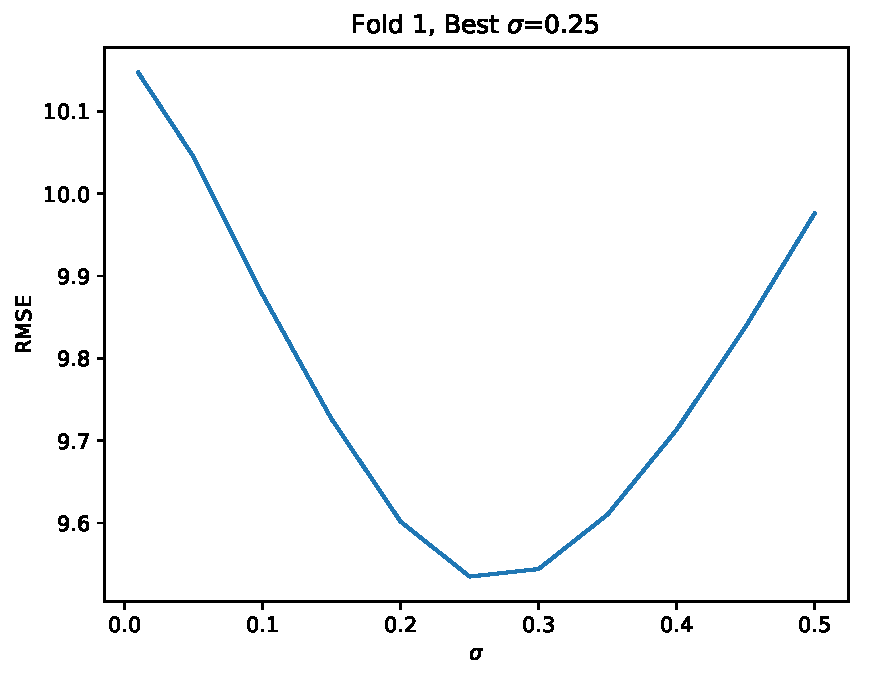
\includegraphics[width=\linewidth]{exercicio2-fold-1.pdf}
		\caption{Fold 1, $\sigma=0.25$}
		\label{fig:exercicio2-fold1}
	\end{subfigure}%
	~ 
	\begin{subfigure}[t]{0.24\textwidth}
		\centering
		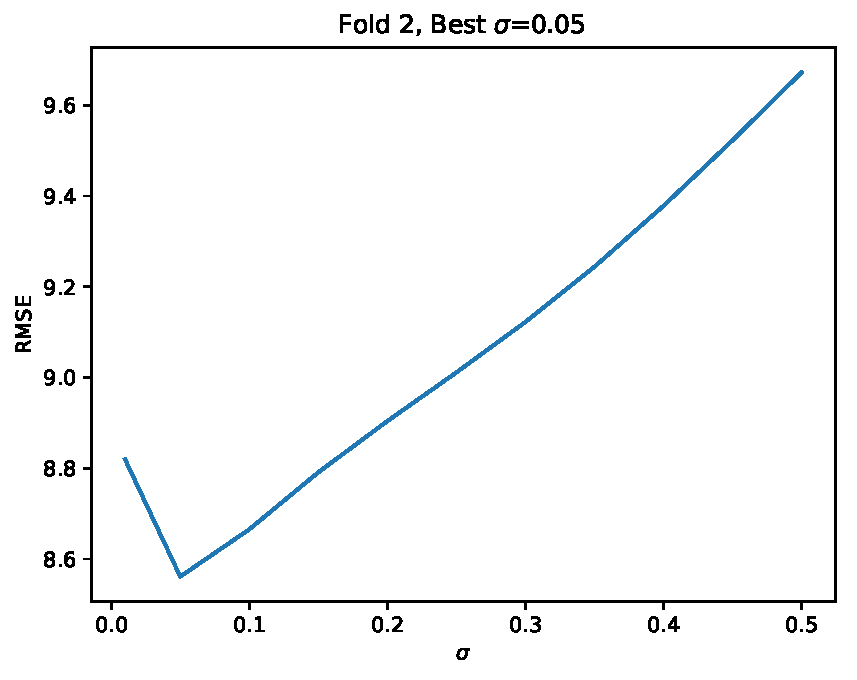
\includegraphics[width=\linewidth]{exercicio2-fold-2.pdf}
		\caption{Fold 2, $\sigma=0.05$}
		\label{fig:exercicio2-fold2}
	\end{subfigure}%
	~
	\begin{subfigure}[t]{0.24\textwidth}
		\centering
		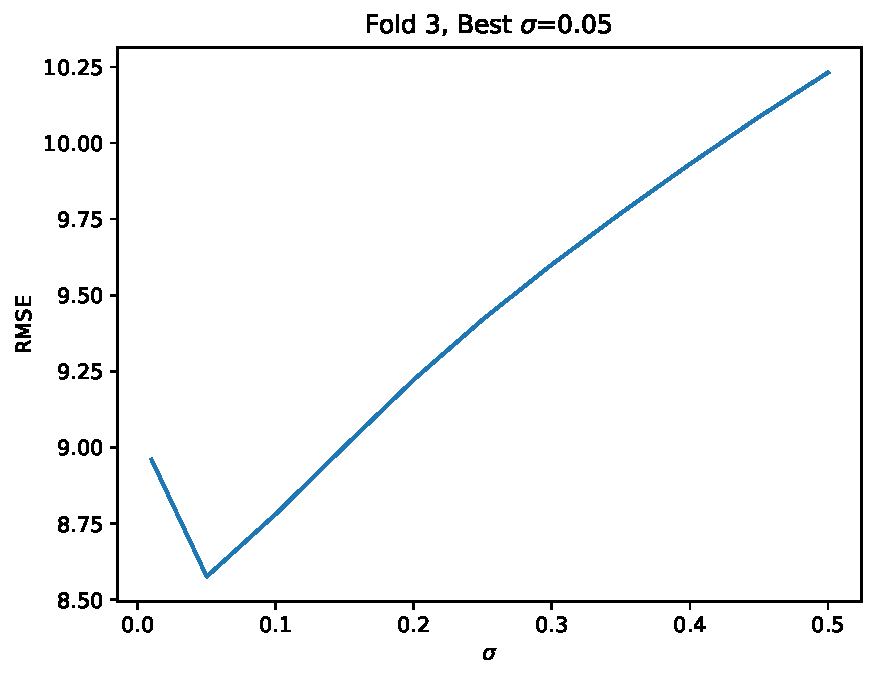
\includegraphics[width=\linewidth]{exercicio2-fold-3.pdf}
		\caption{Fold 3, $\sigma=0.05$}
		\label{fig:exercicio2-fold3}
	\end{subfigure}%
	~
	\begin{subfigure}[t]{0.24\textwidth}
		\centering
		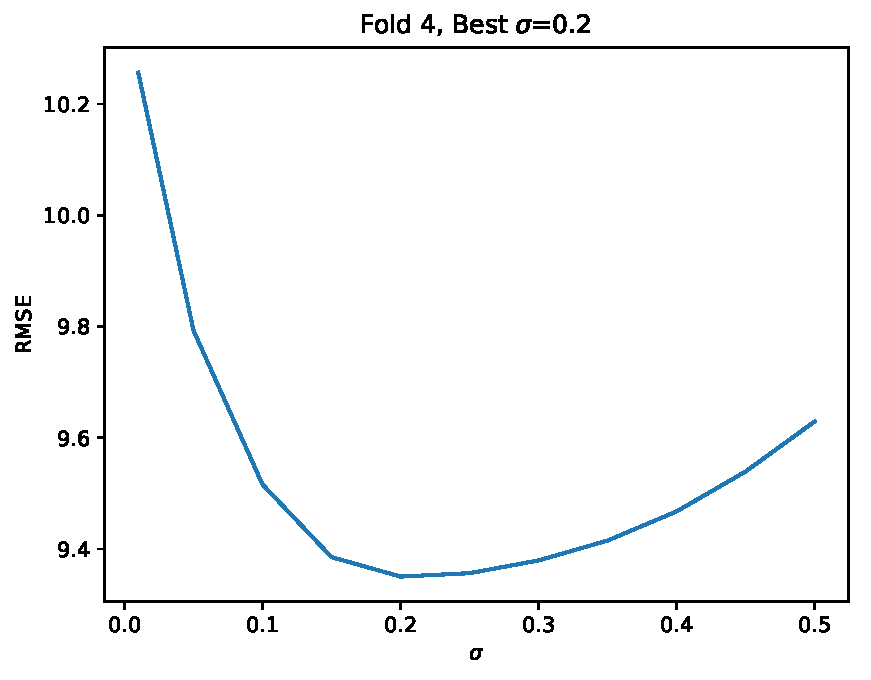
\includegraphics[width=\linewidth]{exercicio2-fold-4.pdf}
		\caption{Fold 4, $\sigma=0.20$}
		\label{fig:exercicio2-fold4}
	\end{subfigure}
	\caption{Calibração do $\sigma$ nos 4 folds.}
	\label{fig:exercicio2}
\end{figure*}

Após a calibração, a GRNN foi retreinada com todo o conjunto de treino inicial (i.e., os 3 folds) e avaliada no conjunto de teste. Os resultados para cada fold podem ser vistos abaixo:

\begin{itemize}
	\item Fold 1, $\sigma=0.25$, RMSE: 8.56
	\item Fold 2, $\sigma=0.05$, RMSE: 8.94
	\item Fold 3, $\sigma=0.05$, RMSE: 9.64
	\item Fold 4, $\sigma=0.20$, RMSE: 8.68
\end{itemize}

\section{Exercício 3}

Realize o teste de Wilcoxon e o teste de sinal com 5\% de nível de significância sobre os dados da \autoref{tab:exercicio3}. Indique se houve alguma técnica que foi estatisticamente superior em cada teste. (Os valores na \autoref{tab:exercicio3} são medidas de acurácia).

\begin{table}[h!]
	\centering
	\caption{Acurácia de 2 classificadores: kNN e kNN++}
	\label{tab:exercicio3}
	\begin{tabular}{@{}cc@{}}
		\toprule
		kNN   & kNN++ \\ \midrule
		66.40 & 84.10 \\
		65.63 & 61.81 \\
		56.95 & 71.98 \\
		64.67 & 75.81 \\
		68.72 & 72.50 \\
		70.37 & 79.71 \\
		61.87 & 78.84 \\
		61.02 & 68.76 \\
		79.64 & 72.95 \\
		51.13 & 60.46 \\
		76.56 & 89.52 \\
		77.40 & 65.02 \\
		73.89 & 63.19 \\
		52.96 & 71.17 \\
		57.86 & 65.94 \\
		60.06 & 74.69 \\
		70.39 & 70.18 \\
		54.10 & 88.55 \\
		71.64 & 87.61 \\
		53.20 & 61.58 \\
		69.61 & 82.14 \\
		64.83 & 68.07 \\
		73.37 & 72.69 \\
		71.45 & 76.44 \\ \bottomrule
	\end{tabular}
\end{table}

Para o teste de Wilcoxon, obtém-se $R^{-}=43$ e $R^{+}=257$, logo $T=\text{min}(R^{-}, R^{+})=43$. Para 24 bases de dados (consultando a tabela disponível no Slide 18 da Aula 10), podemos ver que a hipótese nula é rejeitada com 95\% de confiança (poderia ser rejeitada até mesmo com 99\% de confiança), portanto há uma diferença entre os classificadores comparados. Como o $R^{-}$ foi o menor, podemos dizer que o kNN++ desempenha melhor do que o kNN.

Para o teste de sinal, vemos que o classificador kNN++ é melhor em 18 das 24 bases de dados. Consultando a tabela disponível no Slide 22 da Aula 10, também podemos dizer que o kNN++ desempenha melhor do que o kNN, pois a hipótese nula é rejeitada com 95\% de confiança.


\section*{Instruções para usar os scripts}

O código-fonte enviado foi desenvolvido em Python. Esse código foi testado tanto no Linux (Ubuntu 16.04) quanto no Windows 10. Para rodar os scripts dos exercícios, é necessário ter Python 2.7 ou Python 3.x instalado na sua máquina e algumas dependências. Para instalar as dependências, basta rodar o comando abaixo na raiz do repositório:

\begin{verbatim}
	$ pip install -r lista3/requirements.txt
\end{verbatim}

Para executar o script de um exercicio em específico (por exemplo, o exercício 1), basta executar:

\begin{verbatim}
	$ cd lista3/scripts
	$ python lista3.py --exercicio=1
\end{verbatim}

Ou então, se preferir, você pode executar o script diretamente. Por exemplo:

\begin{verbatim}
	$ cd lista3/scripts
	$ python exercicio1.py
\end{verbatim}

A base de dados Concrete Compressive Strength será baixada automaticamente nas questão em que for usada. Todas as bases de dados estão armazenadas na pasta \texttt{data}. Ao executar os scripts, os gráficos que estão neste relatório serão exibidos e salvos na pasta \texttt{output}. O codigo-fonte desse relatório (em \LaTeX) também se encontra na pasta \texttt{report}. Para garantir a reprodutibilidade dos resultados e gráficos, foi usado como seed o valor \texttt{2017} definido no arquivo \texttt{scripts/constants.py}.

\end{document}
